\documentclass[a4paper]{article}

\usepackage[utf8]{inputenc}
\usepackage[T1]{fontenc}
\usepackage[swedish]{babel}
\usepackage[iso,swedish]{isodate}
\usepackage{icomma}

\usepackage{graphicx}
\usepackage{mathtools}
\usepackage{amsfonts}
\usepackage[hidelinks]{hyperref}
\usepackage[section]{placeins} 
\usepackage{listings}
\lstset{language=matlab, frame=single}

%Setting up how paragraphs are formatted
\setlength{\parindent}{0mm}
\setlength{\itemsep}{0ex}
\setlength{\parskip}{2ex}
\setlength{\parsep}{2ex}
\setlength{\partopsep}{0ex}
\setlength{\topsep}{0ex}
%\addtolength{\topmargin}{}
%\addtolength{\textheight}{}

\addtolength{\oddsidemargin}{-.875in}
\addtolength{\evensidemargin}{-.875in}
\addtolength{\textwidth}{1.75in}

\addtolength{\topmargin}{-.875in}
\addtolength{\textheight}{1.75in}

\title{Transformer, Signaler och System \\ SSY080} 
\author{Erik Thorsell \\ Robert Gustafsson}

\begin{document}
\maketitle

\newpage

\section*{3.1 Fourierserie Uppbyggnad}
\subsection*{a)}
En fyrkantssignal enligt Figur 3 i lab-pm kan betecknas på följande vis:

\[ 
  x(t) =  
    \begin{cases} 
        1   &   \quad 0 < t < \frac{T}{2}\\ 
        -1  &   \quad \frac{T}{2} < t < T\\ 
    \end{cases} 
\] 

För att beräkna Fourierkoefficienterna för signalen använde vi oss av följande
kända uttryck från kurslitteraturen:\\
$2C_k = A_k - jB_k$ (A, B $\in$ $\mathbb{R}$) \\ %\emph{Table 4.2, s.158} \\
$C_k = \frac{1}{T} \int_T x(t)e^{-jkw_{0}t}dt$

Beräkningar följer nedan:
$$ C_k = \frac{1}{T} \int_0^T x(t)e^{-jkw_{0}t}dt = 
\frac{1}{T} \left(\int_0^{\frac{T}{2}} e^{-jkw_{0}t}dt - 
\int_{\frac{T}{2}}^T e^{-jkw_{0}t} dt\right) =$$

$$\frac{1}{T} \left(\left[\frac{e^{-jkw_{0}t}}{-jkw_{0}}\right]_0^{\frac{T}{2}} - 
\left[\frac{e^{-jkw_{0}t}}{-jkw_{0}}\right]_{\frac{T}{2}}^T\right) = $$ 


$$\frac{1}{T} \left(\frac{e^{\frac{-jkw_{0}T}{2}}}{-jkw_{0}} - 
\frac{1}{-jkw_{0}} - \left(\frac{e^{-jkw_{0}T}}{-jkw_{0}} - 
\frac{e^{\frac{-jkw_{0}T}{2}}}{-jkw_{0}}\right)\right) = $$


$$\frac{2e^{\frac{-jkw_{0}T}{2}} - e^{-jkw_{0}T} - 1}{-jkw_{0}T} = $$


$$\frac{1}{-jkw_{0}T}\left(2e^{\frac{-jkw_{0}T}{2}} - e^{-jkw_{0}T} - 1\right) =$$

$$\frac{1}{-jkw_{0}T}\left(2cos\left(\frac{kw_{0}T}{2}\right) - 
2jsin\left(\frac{kw_{0}T}{2}\right) - cos\left(kw_{0}T\right) +
jsin\left(kw_{0}T\right) -1\right) =$$ 

$$\frac{1}{-jk2\pi}(2cos(k\pi) - 2jsin(k\pi) - cos(k2\pi) + jsin(k2\pi)) =$$
$$\begin{cases} 
        \frac{1}{-jk2\pi}(2-1-1)= 0 &   \quad \text{Om k jämn.} \\ 
        \frac{1}{-jk2\pi}(-2-1-1)= \frac{-2j}{k\pi} & \quad \text{Om k udda.}\\ 
\end{cases} 
$$ 
% Om k udda 
%\frac{1}{-jk2\pi}(-2-1-1)= \frac{-4}{-jk2\pi} = \frac{2}{jk\pi} = \frac{-2j}{k\pi} 

$$2C_k = A_k - jB_k $$
$$\text{Eftersom $C_k = 0$ för jämna k } \Rightarrow A_k = 0$$
$$\Rightarrow 2C_k = -jB_k \Rightarrow B_k = -2C_k/j = -2j/k\pi \Leftrightarrow
B_k = \frac{4}{k\pi}$$

\subsection*{b)}
Givet i labpm finns kod för att rita ut en sinusvåg. Genom att modifiera den
koden kan vi genom våra erhållna Fourierkoefficienter rita upp en bättre och
bättre approximation av en fyrkantsvåg. Koden för att beskriva
fyrkantsvågsapproximationen finns nedan och figur~\ref{fig:task1b} visar vår 
approximerade fyrkantsvåg efter summationsindex satt till 100.

\begin{lstlisting}
T=1;
w=2*pi/T;
M=200;
x=0;
t=T*(0:M-1)/M;

for n=1:100
    Ak = 0;
    Bk = 4*mod(n,2)/(n*pi);
    x = x + Ak*cos(n*w*t) + Bk*sin(n*w*t);
end
plot(t,x)
\end{lstlisting}


\section*{3.2 Linjära System och Sinusar}
\subsection*{a)}
Givet i labpm vinns ekvation 12 enligt: 
$G(s) = \frac{(s+0.1)(s+10)}{(s+1)(s^2+s+9)} =
\frac{s^2+10.1s+1}{s^3+2s^2+10s+9}$
detta polynom kan tecknas som täljare och nämnare i Matlab - samt ovandlas till
en överföringsfunktion - med följande kod:

\begin{lstlisting}
num = [1 10.1 1];
den = [1 2 10 9];
Gs=tf(num, den);
\end{lstlisting}

Bode-diagramet samt systemets pol- och nollställen kan ses i
figur~\ref{fig:task2a-bode} och figur~\ref{fig:task2a-pzmap}.

\subsection*{b)}
De tre sinussignalerna ($x1 = sin(t), x2 = sin(3t), x3 = sin(5t)$) finns att
beskåda i figur~\ref{fig:task2b}

\subsection*{c)}
Efter att ha låtit signalerna passera genom vårt givna system ($G(s)$) erhöll
vi tre nya signaler ($y1, y2, y3$) vilka hade förändrad amplitud och fas
gentemot vår insignal. Detta var givetvis väntat. Den svarta kurvan visar
insignalen och den blå visar signalen vilken returnerades av lsim. Vidare
beräknade vi även amplitud och fas var och en för sig varefter vi lät den
signalen gå genom systemet för att erhålla en signal lika med den som erhölls
av lsim. Detta för att bekräfta ekvation 2 i labpm.

Koden för att bekräfta ekv 2 kan ses nedan:

\begin{lstlisting}
phi1 = angle(evalfr(Gs,1j));
x1p = sin(t+phi1);
y1p = abs(evalfr(Gs,1j))*x1p;

phi2 = angle(evalfr(Gs,3j));
x2p = sin(3*t+phi2);
y2p = abs(evalfr(Gs,3j))*x2p;

phi3 = angle(evalfr(Gs,5j));
x3p = sin(5*t+phi3);
y3p = abs(evalfr(Gs,5j))*x3p;
\end{lstlisting}

Här kommer $y1p, y2p \text{ samt } y3p$ vara lika med $y1, y2 \text{ och } y3$
vilka erhölls från lsim och vi ser alltså att ekv 2 stämmer.


\section*{3.3 Periodiska Insignaler och DFT}
\subsection*{a)}
För att generera och rita upp en fyrkantsvåg i Matlab använde vi oss av
följande kod:

\begin{lstlisting}
N = 2.^13;
F = 100;
Ts = 1/F;
t = 0:Ts:40*pi;
x = square(t);
plot(t, x)
\end{lstlisting}

Den resulterande grafen, samt dess fourierkoefficienter (vilka ska räknas ut i
senare uppgifter) finns att finna i figur~\ref{fig:task3c-square-+-fk}.
Eftersom $x(t) = -x(-t)$ ser vi att signalen är udda.

\subsection*{b)}
De tre första - nollskilda - fourierkoefficienterna för fyrkantsvågen är: 
1.2732, 0.4244, 0.2546 och beräknades med hjälp av $B_k = \frac{4}{k\pi}$ där
$k=1,3,5$.

\subsection*{c)}
Genom att använda den snabba fouriertransformen (den inbyggda matlabfunktionen
\emph{fft}) kunde vi beräkna den diskreta fouriertransformen av fyrkantsvågen.
Grafen till uppgiften återfinns i figur~\ref{fig:task3c-square-+-fk} vilket är
samma figur som i uppgift a).\\\\
Spektrumet består av $\omega_k = 1, 3, 5$ och det går även att skymta $\omega_k =
7$.

\subsection*{d)}
Genom att använda sambandet i ekvation 10 ($B=\frac{2|X[k_0]|}{N}$) i labpm kunde
vi beräkna de praktiska värdena för fourierkoefficienterna vi tog fram i uppgift
b. Resultatet för de båda ges i tabellen nedan.

\begin{tabular}{| l | l | l | l |}
    \hline
     & 1 & 3 & 5 \\ \hline
    Teoretiska & 1.2732 & 0.4244 & 0.2546 \\ \hline
    Praktiska & 1.2702 & 0.4154 & 0.2398 \\ \hline
\end{tabular}

\subsection*{e)}
Fyrkantssignalen applicerades på $G(s)$ varefter de tre första
fourierkoefficienterna bestämdes teoretiskt med hjälp av ekvation 8 i labpm.
Ekvation 8 lyder som bekant: $y(t) = A_0 g(0) + \sum_{k=1}^{\infty} B_k
g(k\omega_0)sin(k\omega_0t+\Phi(k\omega_0))$. Då $g(w) = |G(jw)|$ och $B_k$ är
fourierkoefficienten för insignalen kan vi beräkna fourierkoefficienten för
utsignalen vid ett givet $k$ med hjälp av:

\begin{lstlisting}
abs(evalfr(H,kj))*(4/k*pi)
\end{lstlisting}

Därefter användes återigen den snabba fouriertransformen för att beräkna
koefficienterna i praktiken. En tabell med värdena ges nedan och i
figur~\ref{fig:task3d+fk} ges återigen spektrumet för fyrkantsvågen i
frekvensdomänen samt spektrumet för utsignalen när fyrkantsvågen applicerats på
systemet $G(s)$.\\\\
Eftersom ett system bara kan förändra en signals amplitud och fas är spektrum
oförändrat före och efter det att systemet har applicerats på signalen.

\begin{tabular}{| l | l | l | l |}
    \hline
     & 1 & 3 & 5 \\ \hline
    Teoretiska & 1.1279 & 1.4020 & 0.1666 \\ \hline
    Praktiska & 1.023 & 1.3378 & 0.1513 \\ \hline
\end{tabular}


\section*{3.4 Notch-filter}
\subsection*{a)}
Polynomet vilket söks i uppgiften är 
$Ts = s*(s-1j)*(s+1j)*(s-5j)*(s+5j)*(s-7j)*(s+7j)*(s-9j)*(s+9j)$ där
komplexkonjugerade nollställen används för att få ett polynom med reella
koefficienter. Om man låter nämnaren vara lika med 1 och använder Matlabs
inbyggda funktion för att generera en överföringsfunktion kan det resulterande
systemet visas med hjälp av ett Bodediagram. Detta diagram finns att beskåda i
figur~\ref{fig:task4a-bode}.

\subsection*{b)}
Efter att ha provat oss fram drog vi slutsatsen att 10 stycken poler sådana att
$p=-4$ var lämpliga för att dämpa höga frekvenser med systemet. Bodediagramet
finns att se i figur~\ref{fig:task4b-bode}.

\subsection*{c)}
För att gå en dämpning på 60 dB för vinkelfrekvenser $\omega \gg 9
\frac{\text{rad}}{s}$ erfodrades 11 poler.

\subsection*{d)}
För att förstärka vårat system skalade vi täljarpolynomet med $|H(j3)|$.
Filtrets frekvenssvar finns återgivet i figur~\ref{fig:task4d-bode}.

\subsection*{e)}
Det finns massor med bilder längst ner!


\clearpage

\begin{figure}
    \caption{Fyrkantsvåg för uppgift 3.1 b).}
    \centering
    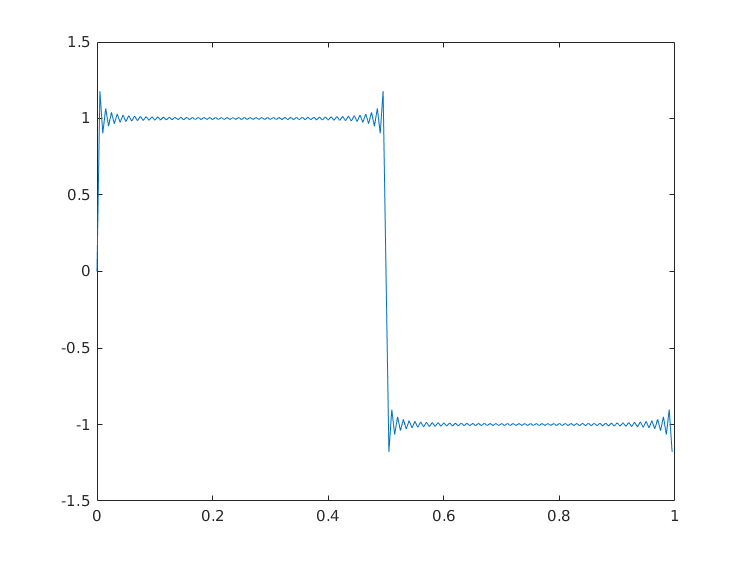
\includegraphics[scale=0.75]{figures/task1b.png}
    \label{fig:task1b}
\end{figure}

\begin{figure}
    \caption{Bodediagram för G(s).}
    \centering
    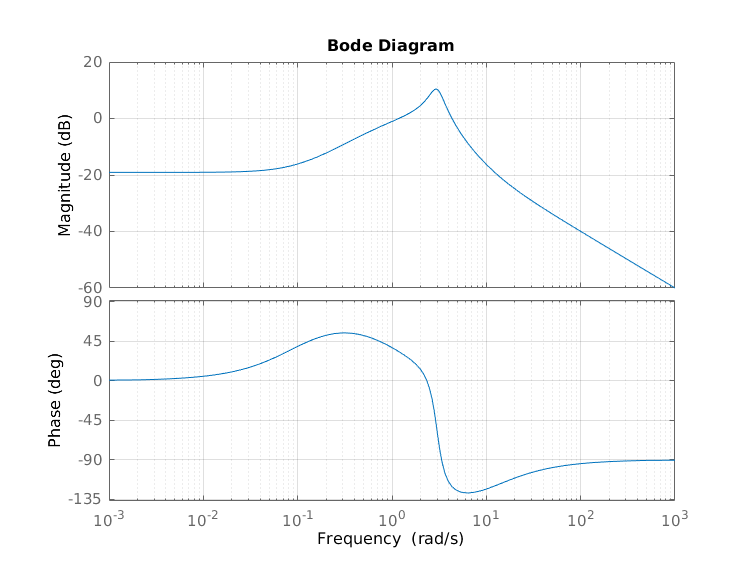
\includegraphics[scale=0.8]{figures/task2a-bode.png}
    \label{fig:task2a-bode}
\end{figure}

\begin{figure}
    \caption{Nod- och polgraf för G(s).}
    \centering
    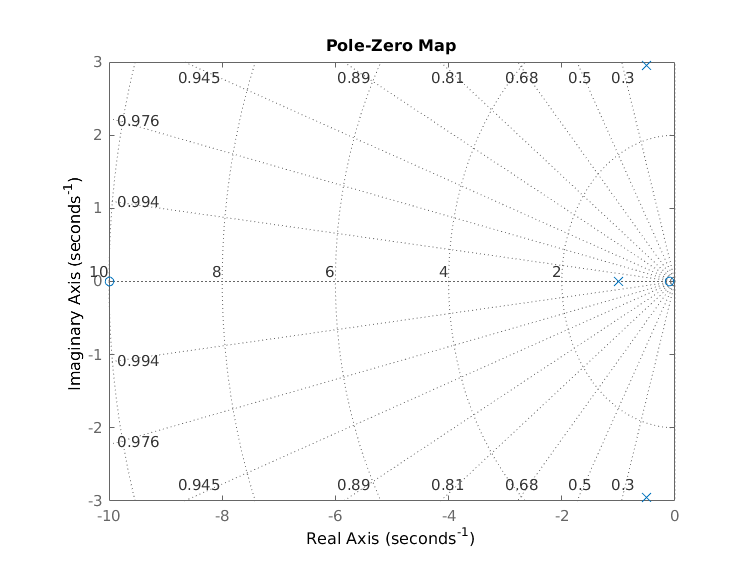
\includegraphics[scale=0.8]{figures/task2a-pzmap.png}
    \label{fig:task2a-pzmap}
\end{figure}

\begin{figure}
    \caption{De tre insignalerna givna i uppgift 3.2 b).}
    \centering
    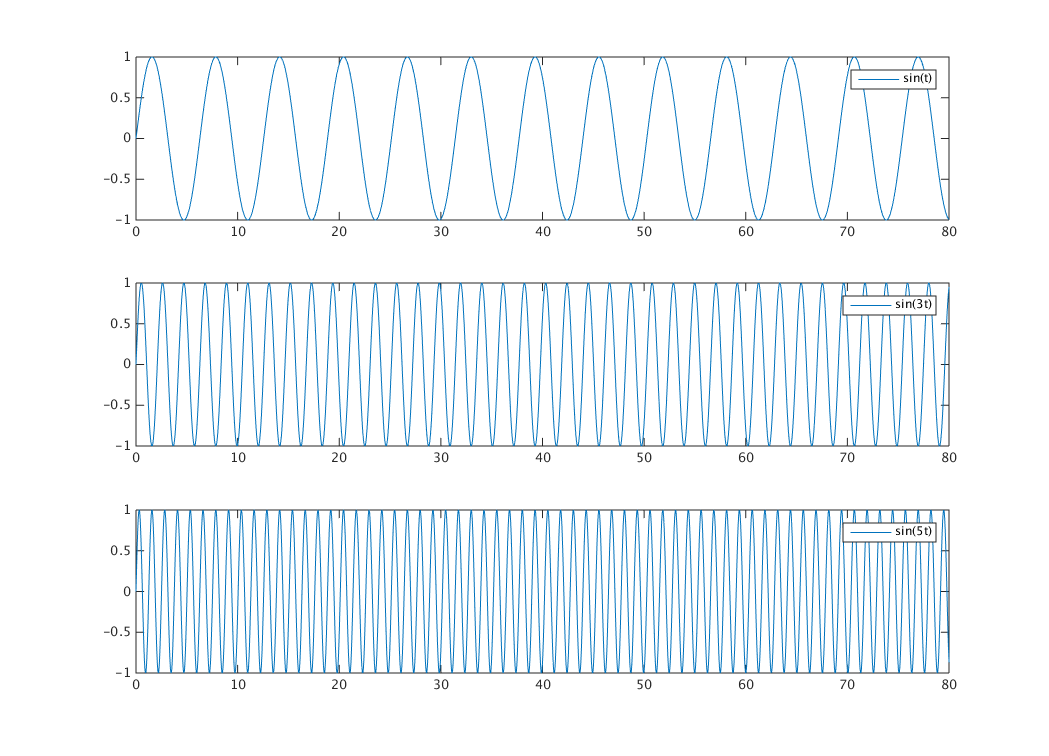
\includegraphics[scale=0.55]{figures/task2b.png}
    \label{fig:task2b}
\end{figure}

\begin{figure}
    \caption{Utsignaler samt insignal för uppgift 3.2 c).}
    \centering
    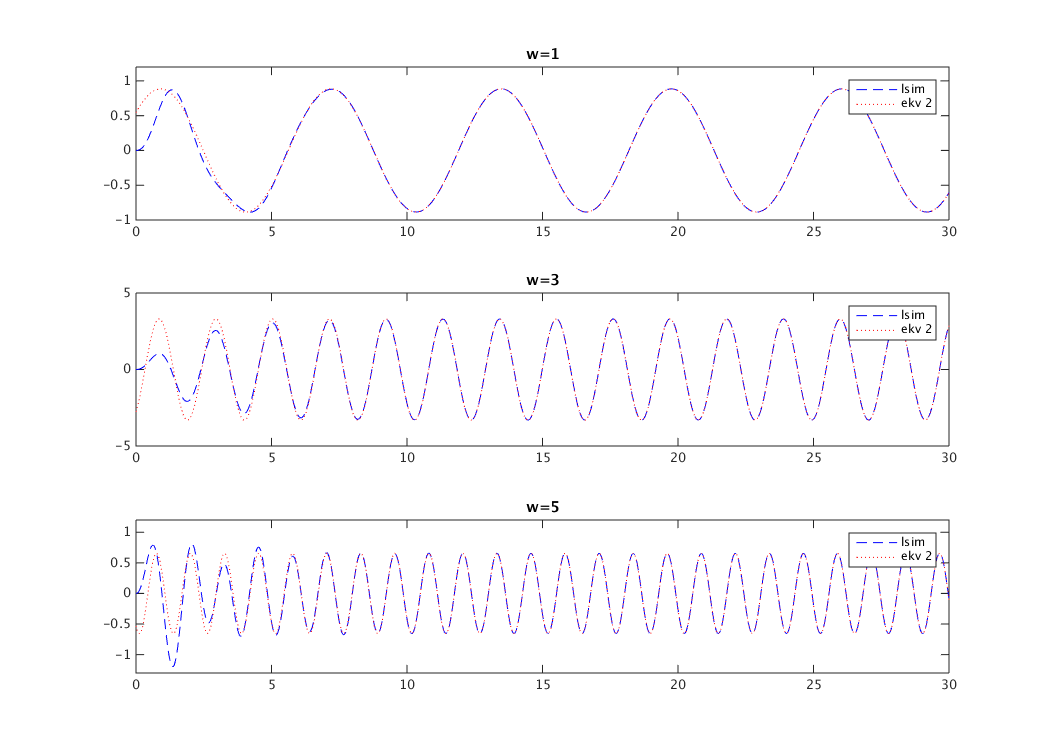
\includegraphics[scale=0.55]{figures/task2c-three-waves.png}
    \label{fig:task2c-three-waves}
\end{figure}

\begin{figure}
    \caption{En, av matlab genererad, fyrkantsvåg samt spektrumet för dess
    snabba fouriertransform med avseende på $\omega_k$.}
    \centering
    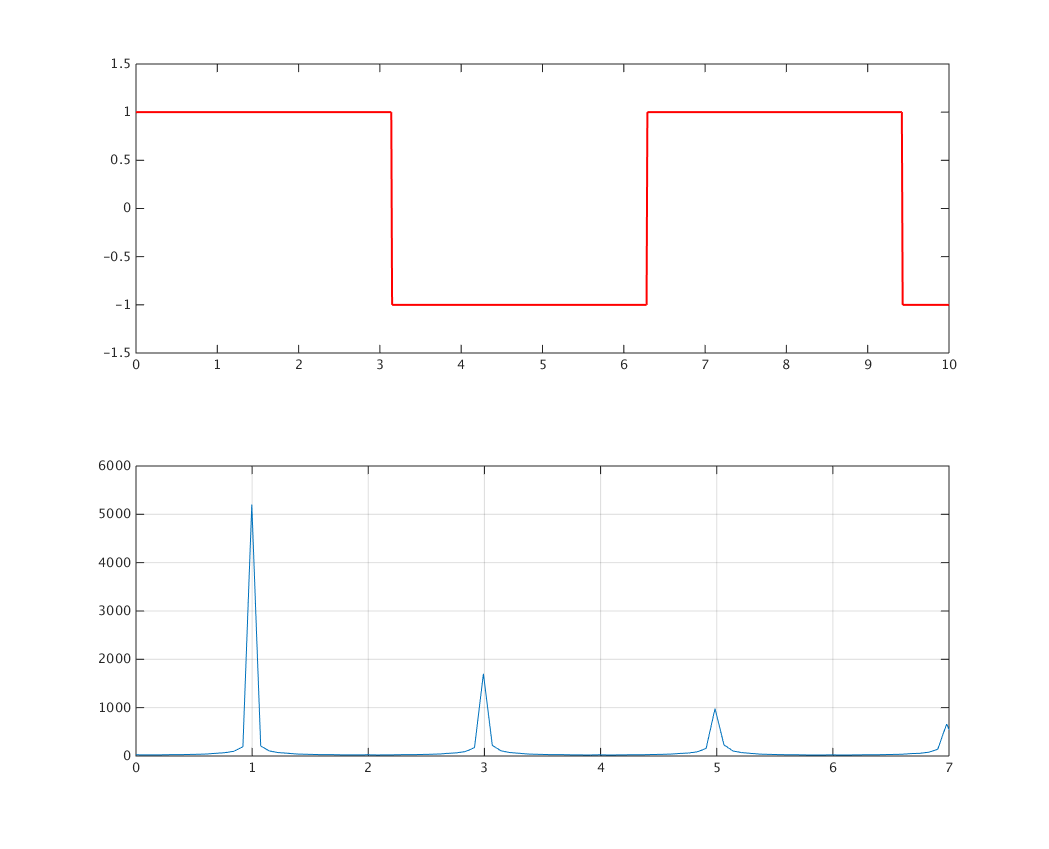
\includegraphics[scale=0.55]{figures/task3c-square-+-fk.png}
    \label{fig:task3c-square-+-fk}
\end{figure}

\begin{figure}
    \caption{De tre första - nollskiljda - fourierkoefficienterna för
    fyrkantsvågen samt för utsignalen som ges när
    fyrkantsvågen passerar systemet G(s).}
    \centering
    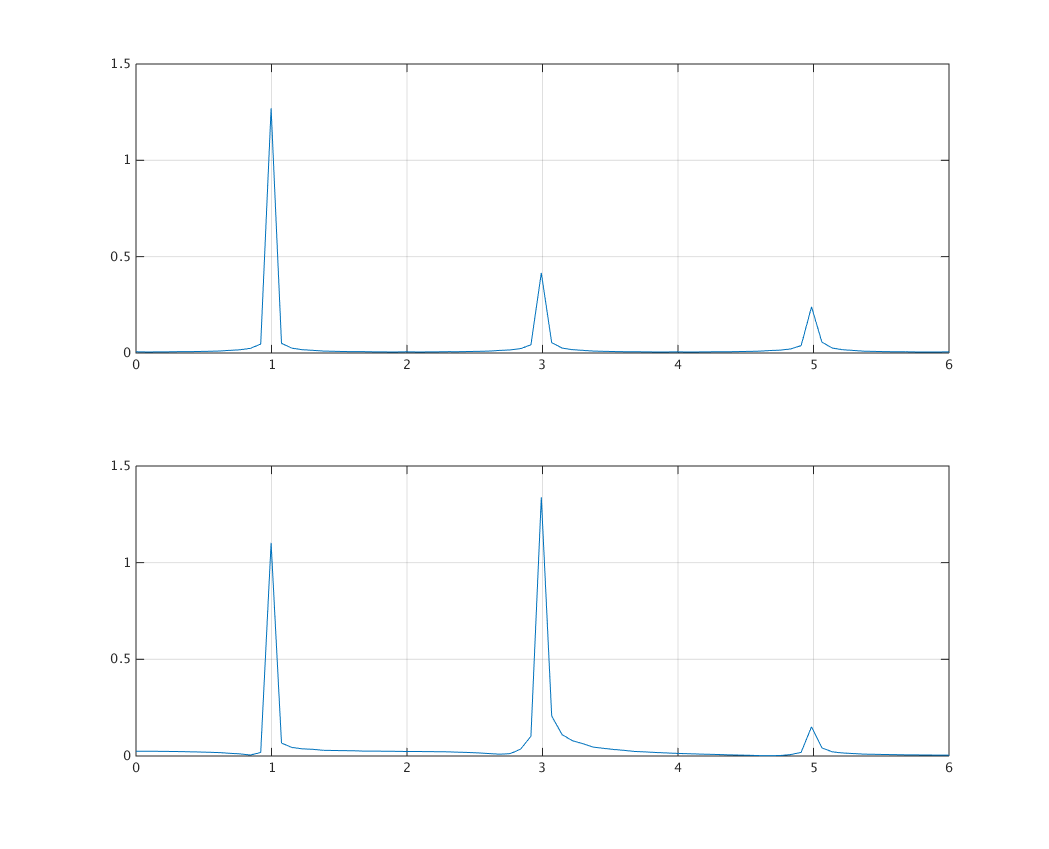
\includegraphics[scale=0.55]{figures/task3d+fk.png}
    \label{fig:task3d+fk}
\end{figure}

\begin{figure}
    \caption{Bodediagram för vårt egentillverkade system enligt uppgift 3.4 a).}
    \centering
    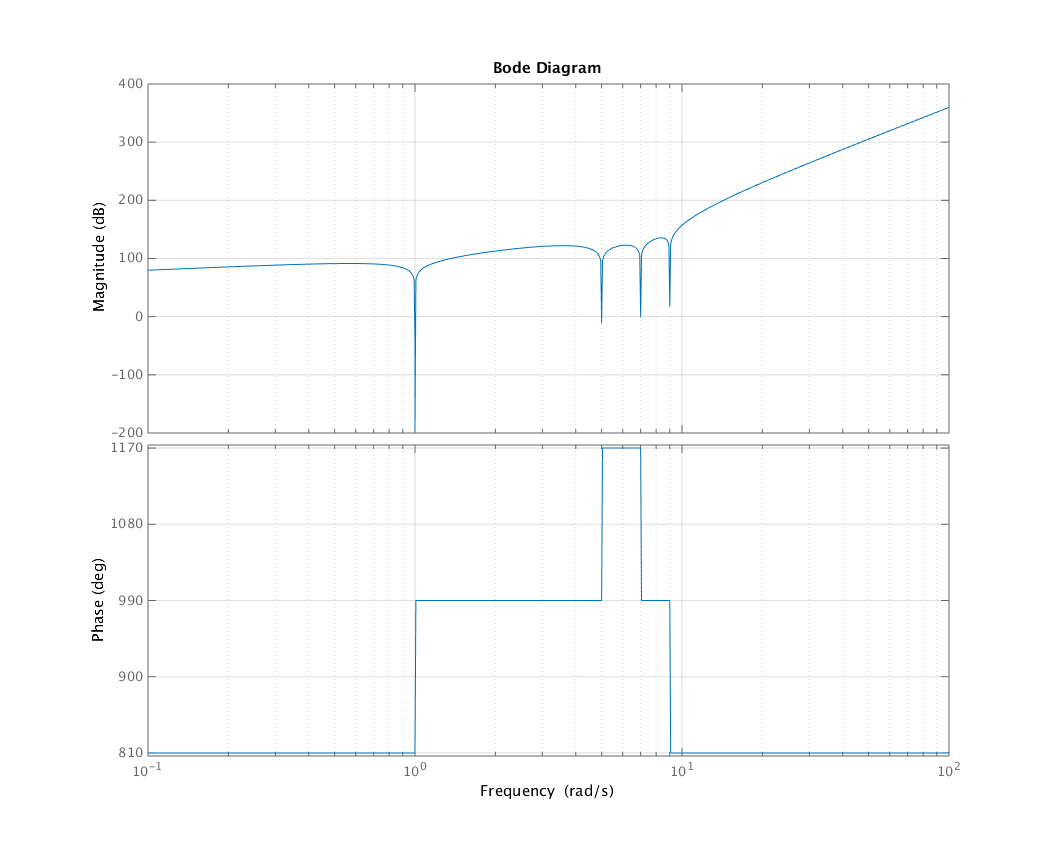
\includegraphics[scale=0.55]{figures/task4a-bode.png}
    \label{fig:task4a-bode}
\end{figure}

\begin{figure}
    \caption{Bodediagram som visar systemet efter att $\omega > 9$ dämpats.}
    \centering
    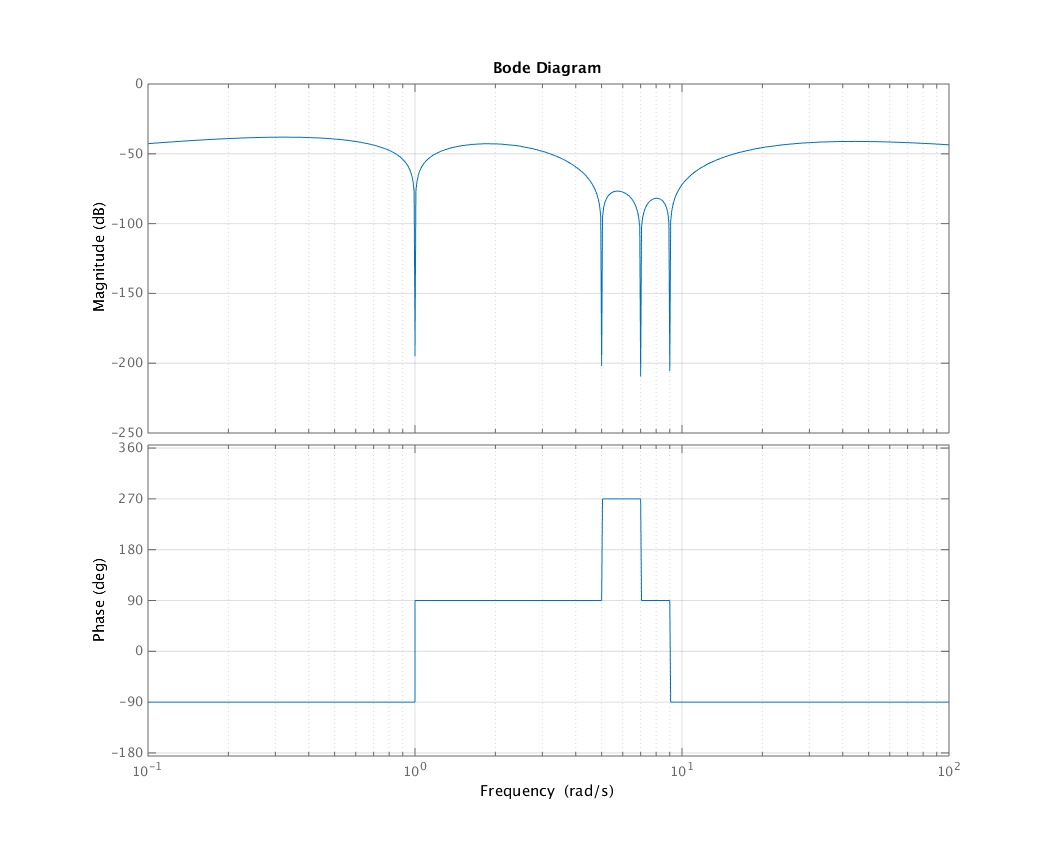
\includegraphics[scale=0.55]{figures/task4b-bode.png}
    \label{fig:task4b-bode}
\end{figure}

\begin{figure}
    \caption{Bodediagram som visar systemet efter att $\omega \gg 9$ dämpats.}
    \centering
    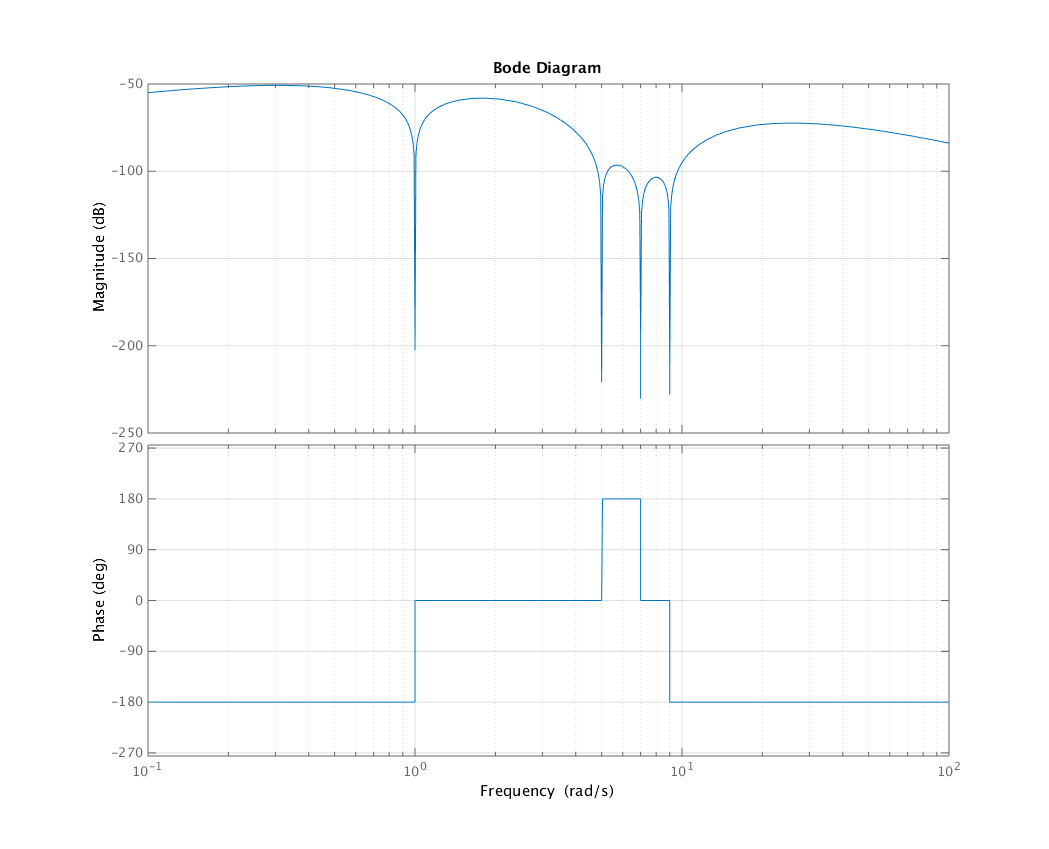
\includegraphics[scale=0.55]{figures/task4c-bode.png}
    \label{fig:task4c-bode}
\end{figure}

\begin{figure}
    \caption{Bodediagram som visar vårt system innan amplitudkorrigering i
    blått och det slutliga systemet i rött.}
    \centering
    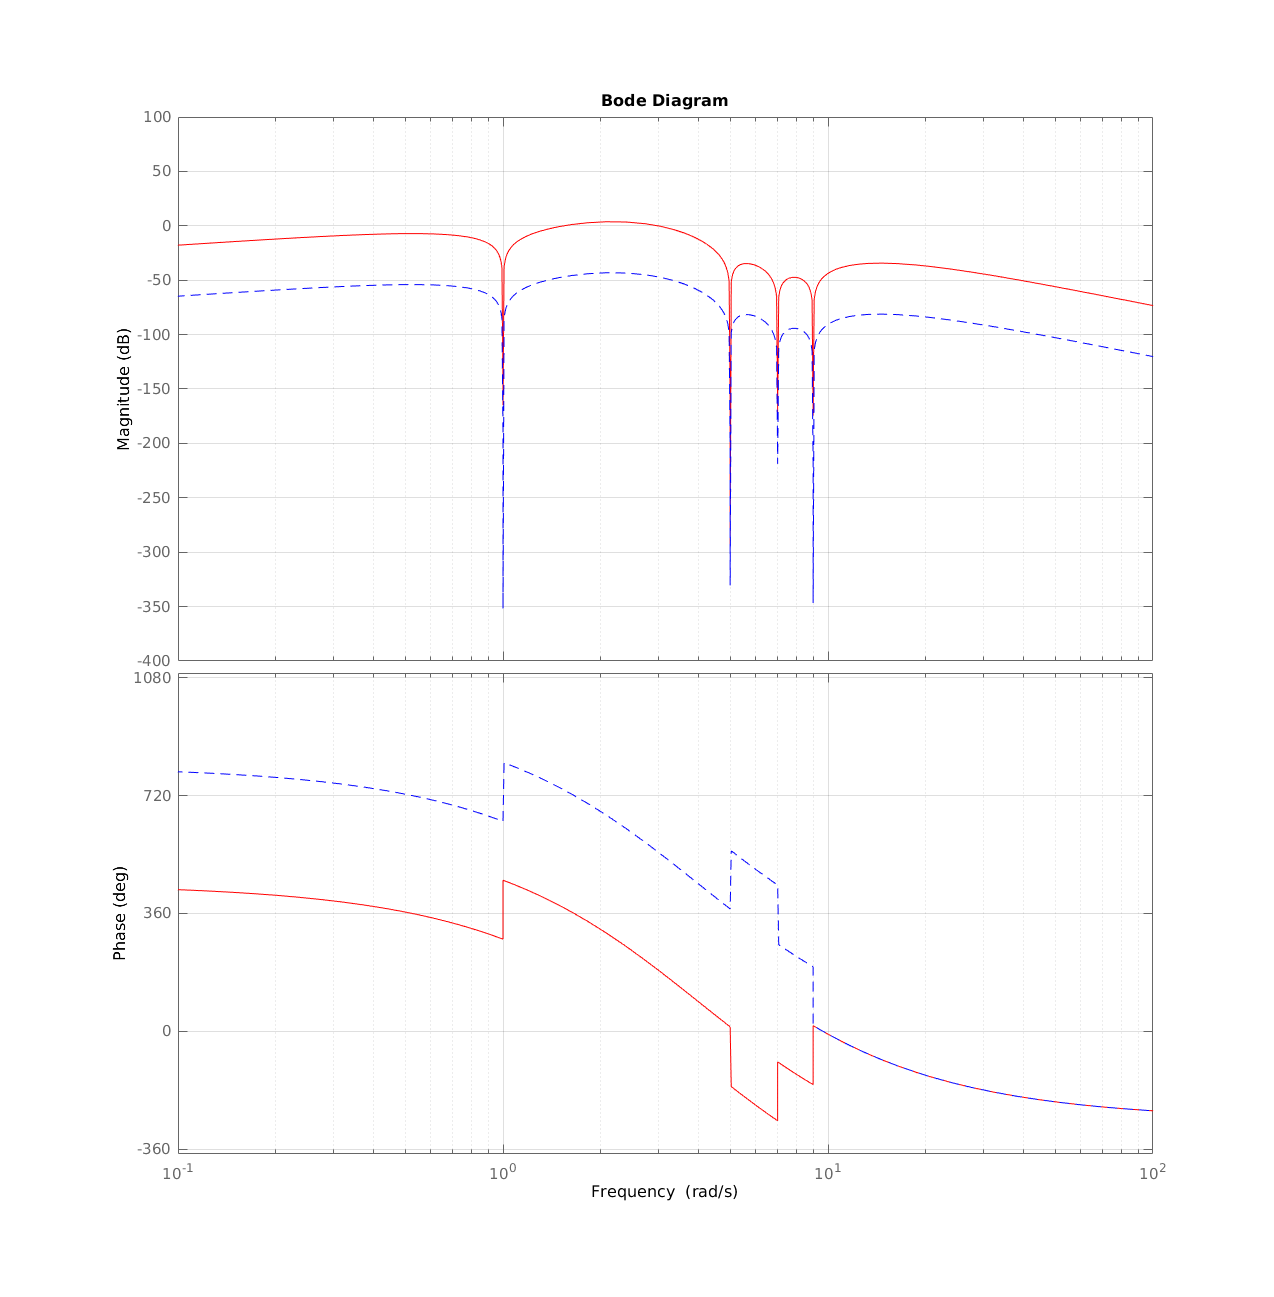
\includegraphics[scale=0.55]{figures/task4d-bode.png}
    \label{fig:task4d-bode}
\end{figure}

\clearpage

\begin{figure}
    \caption{När x-signalen passerat systemet synns tydligt att frekvensvinkeln
    $\omega = 3$ och signalen är tydligt sinusformad.}
    \centering
    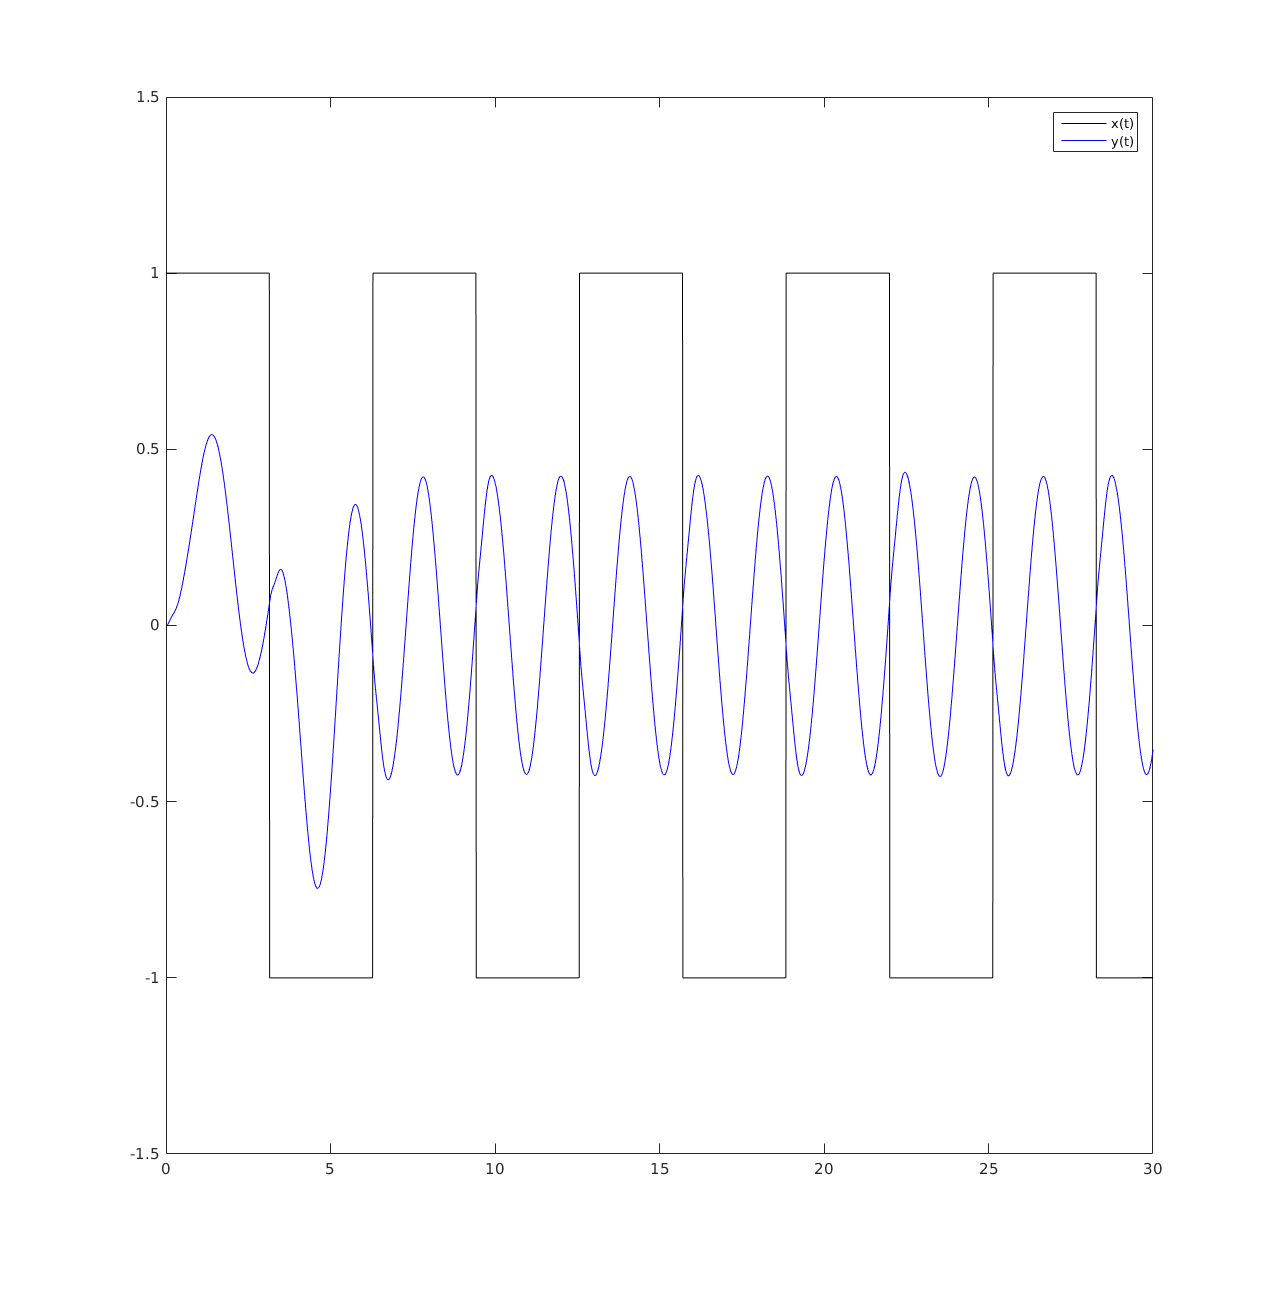
\includegraphics[scale=0.55]{figures/task4e-xsignal-sys2.png}
    \label{fig:task4e-xsignal-sys2}
\end{figure}

\begin{figure}
    \caption{När y-signalen (fyrkantsvågen som först passerat G(s) och sedan
    vårt notchfilter) slutligen ritas upp återfinns den förväntade
    vinkelfrekvensen och sinuskarraktären.}
    \centering
    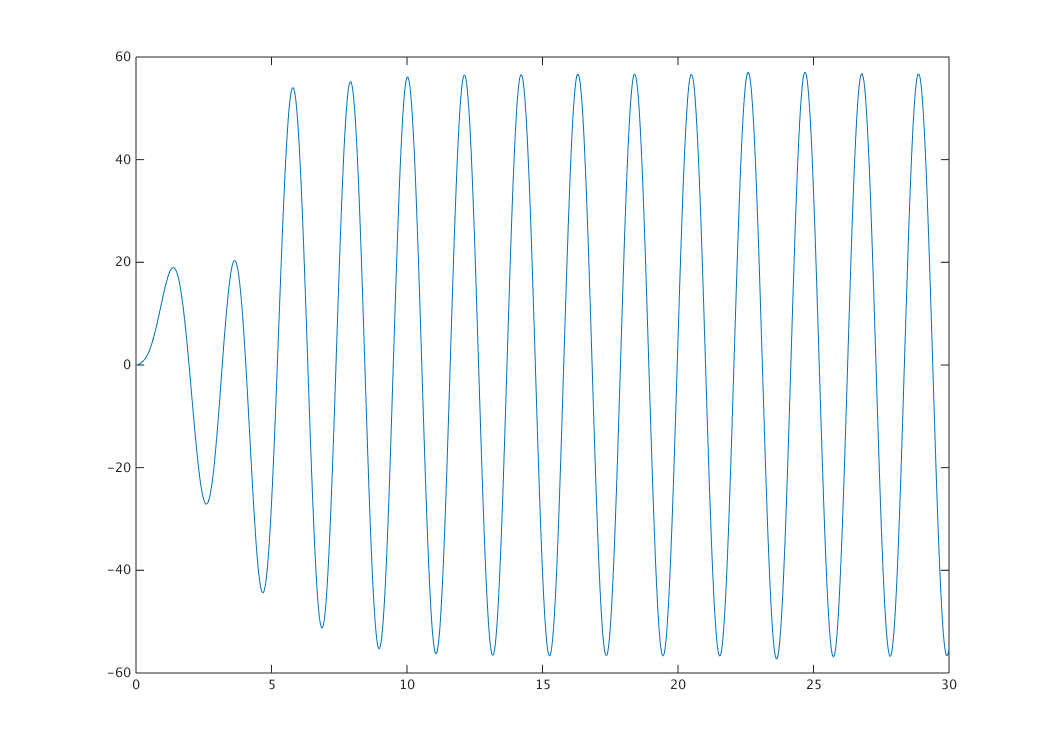
\includegraphics[scale=0.55]{figures/task4e-y-sys2.png}
    \label{fig:task4e-y-sys2}
\end{figure}

\begin{figure}
    \caption{Här ses tydligt att $\omega = 3$ släpps igenom.}
    \centering
    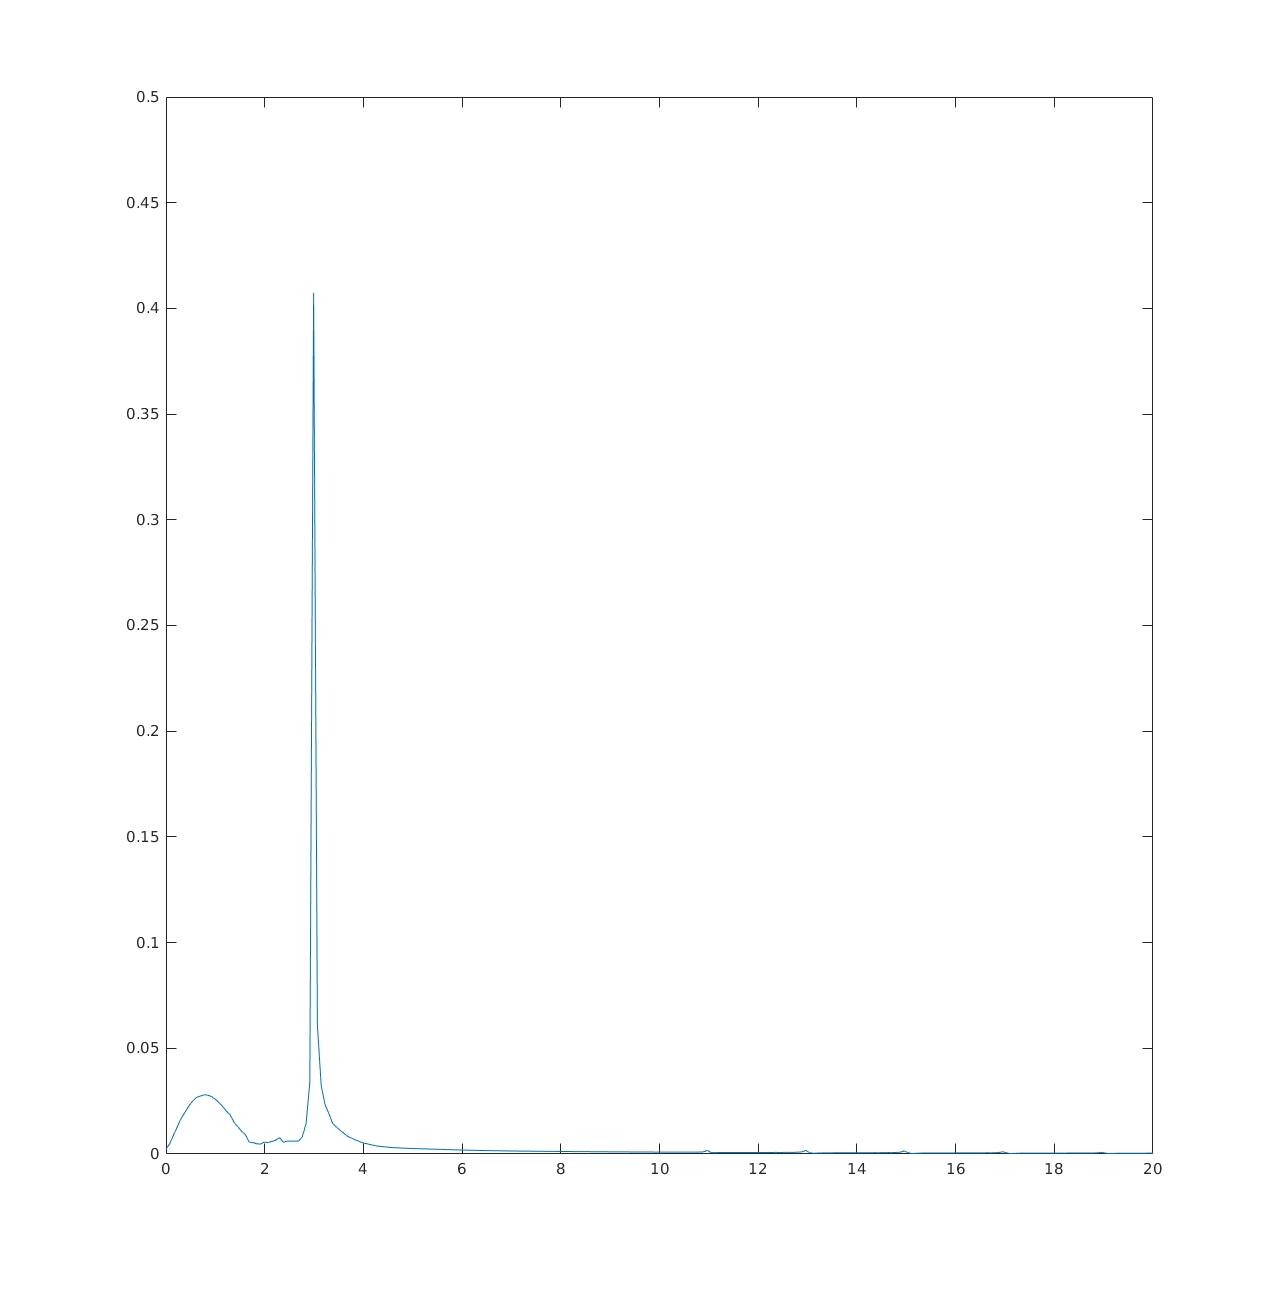
\includegraphics[scale=0.5]{figures/task4e-fk-x-sys2.png}
    \label{fig:task4e-fk-x-sys2}
\end{figure}

\begin{figure}
    \caption{Även här släpps $\omega = 3$ igenom som brukligt.}
    \centering
    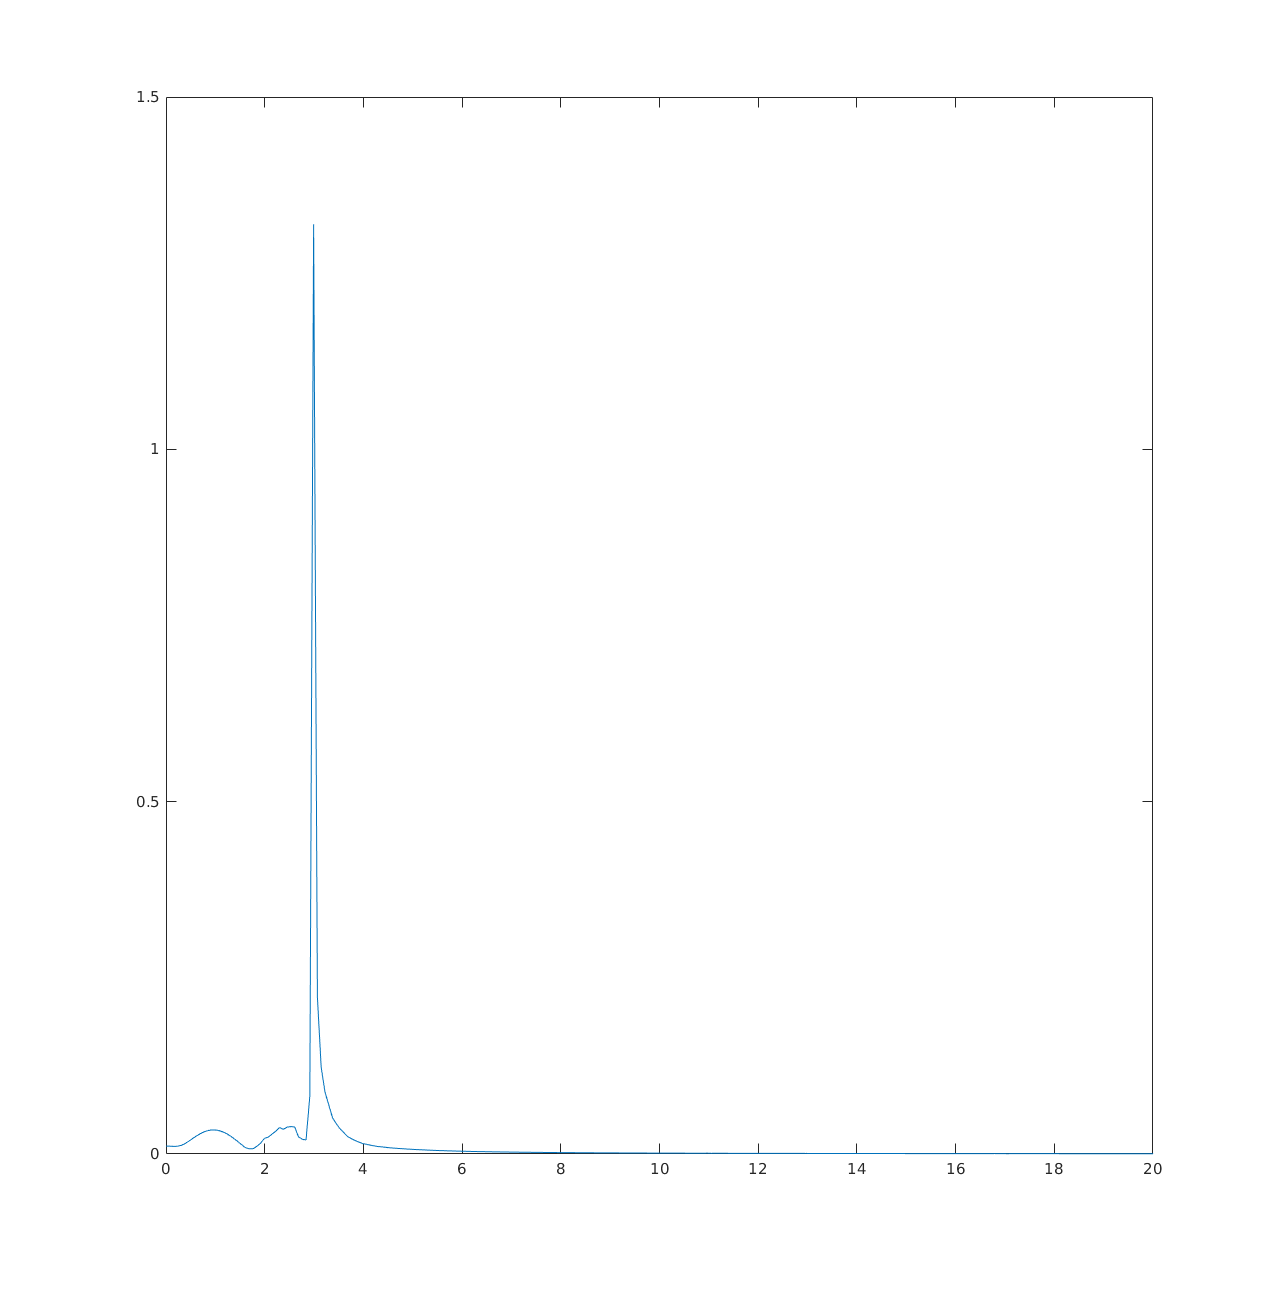
\includegraphics[scale=0.5]{figures/task4e-fk-y-sys2.png}
    \label{fig:task4e-fk-y-sys2}
\end{figure}





\clearpage

\appendix
\begin{lstlisting}
%% Uppgift 3.1 a)

% An = 0
% Bn = 4/(k*pi)
% Se fk.tex

% Uppgift 3.1 b)
clf
clc
syms n x k

T=1;
w=2*pi/T;
M=200;
x=0;
t=T*(0:M-1)/M;

for n=1:100
    Ak = 0;
    Bk = 4*mod(n,2)/(n*pi);
    x = x + Ak*cos(n*w*t) + Bk*sin(n*w*t);
end
plot(t,x)

%% Uppgift 3.2 a)
clf
clc

% y(t) = g(w)sin(wt+phi(w))
% num  = (s^2+10.1s+1)
% den  = (s^3+2*s^2+10*s+9)

num = [1 10.1 1];
den = [1 2 10 9];
Gs=tf(num, den);

% Uppgift 3.2 b)
F=100;
N=2.^13;
Ts=1/F;
Tmax = (N-1)*Ts;
t=0:Ts:Tmax; 

% Insignals
x1 = sin(t);
x2 = sin(3*t);
x3 = sin(5*t);

% % Plots
% subplot(3,1,1)
% plot(t, x1)
% legend('sin(t)')
% axis([0 80 -1 1])
% subplot(3,1,2)
% plot(t, x2)
% legend('sin(3t)')
% axis([0 80 -1 1])
% subplot(3,1,3)
% plot(t, x3)
% legend('sin(5t)')
% axis([0 80 -1 1])

% Uppgift 3.2 c)

% y = x sent through sys using lsim
y1 = lsim(Gs,x1,t);
y2 = lsim(Gs,x2,t);
y3 = lsim(Gs,x3,t);

% y = correct amplitude, wrong phase
y1e = abs(evalfr(Gs,1j))*x1;
y2e = abs(evalfr(Gs,3j))*x2;
y3e = abs(evalfr(Gs,5j))*x3;

% y = correct amp and phase due to eq 2
phi1 = angle(evalfr(Gs,1j));
x1p = sin(t+phi1);
y1p = abs(evalfr(Gs,1j))*x1p;

phi2 = angle(evalfr(Gs,3j));
x2p = sin(3*t+phi2);
y2p = abs(evalfr(Gs,3j))*x2p;

phi3 = angle(evalfr(Gs,5j));
x3p = sin(5*t+phi3);
y3p = abs(evalfr(Gs,5j))*x3p;

% % % Plots
% % a)
% bode(sys)
% pzmap(sys)

% c)
subplot(3,1,1)
plot(t,y1,'--b', t,y1p,':r', t, x1,'k')
axis([0 30 -1 1.2])
legend('lsim1', 'ekv 2', 'x1'), title('w=1')

subplot(3,1,2)
plot(t,y2, '--b', t, y2p, ':r',t, x2,'k')
axis([0 30 -5 5])
legend('lsim2', 'ekv 2','x2'), title('w=3')

subplot(3,1,3)
plot(t,y3, '--b', t, y3p, ':r',t,x3,'k')
axis([0 30 -1.3 1.2])
legend('lsim3', 'ekv 2','x3'), title('w=5')

%% Uppgift 3.3 a)
clf
clc

N = 2.^13;
F = 100;
Ts = 1/F;
t = 0:Ts:40*pi;
x = square(t);
% x(t) != x(-t) => x ar udda

% Uppgift 3.3 b)
fprintf('3.3 b\n')
fprintf('FK enligt ekv 1:\n\n')
for n = 1:5;
    An = 0;
    Bn = 4*mod(n,2)/(n*pi);
    if(Bn)
        disp(Bn)
    end
end

% Uppgift 3.3 c)
k = 0:(N-1);
wk = (2*pi*F*k)/(N);
kf=@(wk) (N*wk)/(2*pi*F);
ffx=fft(x, N);

% Uppgift 3.3 d)
B1 = (2*abs(ffx(k+1)))/N;
fprintf('3.3 d\n')
fprintf('FK enligt fft (ekv 10):\n\n')
B1max1 = max((B1(1:ceil(kf(2)))));
B1max2 = max((B1(ceil(kf(2)):ceil(kf(4)))));
B1max3 = max((B1(ceil(kf(4)):ceil(kf(6)))));
disp(B1max1)
disp(B1max2)
disp(B1max3)

% Uppgift 3.3 e)
num = [1 10.1 1];
den = [1 2 10 9];
H=tf(num, den);

y = lsim(H,x,t);

%plot(t, y);

% Enligt ekv 8
fprintf('3.3 e\n')
fprintf('FK enligt ekv 8:\n\n')
disp(abs(evalfr(H,1j))*4/(pi*1))
disp(abs(evalfr(H,3j))*4/(pi*3))
disp(abs(evalfr(H,5j))*4/(pi*5))

% Enligt fft
ffy = fft(y, N);
B2 = (2*abs(ffy(k+1)))/N;

fprintf('FK enligt fft (ekv 10):\n\n')
B2max1 = max((B2(1:ceil(kf(2)))));
B2max2 = max((B2(ceil(kf(2)):ceil(kf(4)))));
B2max3 = max((B2(ceil(kf(4)):ceil(kf(6)))));
disp(B2max1)
disp(B2max2)
disp(B2max3)

% Plots
subplot(3,1,1)
plot(t, x, 'r', 'linewidth', 1.5)
axis([-0 10 -1.5 1.5])
grid on
subplot(3,1,2)
plot(wk, abs(ffx))
axis([0 6 0 6000])
grid on
subplot(3,1,3)
plot(wk, abs(B2))
axis([0 6 -0 1.5])
grid on

%% Uppgift 3.4 a)
clc
clf

syms s;

Ts = s*(s-1j)*(s+1j)*(s-5j)*(s+5j)*(s-7j)*(s+7j)*(s-9j)*(s+9j);
num = [1 0 156 0 7374 0 106444 0 99225 0];
Tp = tf(num, 1);
% % Plots
%bode(Tp);
%grid on

% Uppgift 3.4 b: n=10, c: n=11)
Np = 1;
for n = 1:12
    Np = Np*(s+4);
end
den = sym2poly(Np);
sys = tf(num,den);
w={1,5000};
% % Plots
%bode(sys,w);
%grid on

% Uppgift 3.4 d)
scale = abs(evalfr(sys, 3j));
sys2 = tf(num/scale, den);
abs(evalfr(sys2,3j));
% % Plots
% bode(sys2, 'r');
% grid on
% hold on
% bode(sys, '--b');

% Uppgift 3.4 e)
N=8192;
k = 0:(N-1);
wk = (2*pi*F*k)/(N);
F = 100;
Ts = 1/F;
t = 0:Ts:(N-1)*Ts;
x = square(t);

% x=square(t)
yx = lsim(sys2,x,t);
ffy = fft(yx, 8192);
By = (2*abs(ffy(k+1)))/N;
% % Plots
% plot(t,x, 'k', t, yx, 'b');
% legend('x(t)', 'y(t)')
% axis([0 30 -1.5 1.5])
% plot(wk, abs(By));
% axis([0 20 0 .5])


% % Amplitud hos Notchfiltrets utsignal
% fprintf('Notch-amp square:')
% disp(max(yx))
% % Amplitud genom DTF och FFT
% fprintf('FFT-amp square:')
% disp(max(By))

% ysignalen
num = [1 10.1 1];
den = [1 2 10 9];
H=tf(num, den);
y = lsim(H,x,t);
yy = lsim(sys2, y,t);
ffy = fft(yy, 8192);
By = (2*abs(ffy(k+1)))/N;
% % Plots
% plot(t,y, 'k', t, yy);
% legend('x(t)', 'y(t)')
% axis([0 30 -3 3])
plot(wk, abs(By));
axis([0 20 0 1.5])

% % Amplitud hos Notchfiltrets utsignal
% fprintf('Notch-amp yy:')
% disp(max(yy))
% % Amplitud genom DTF och FFT
% fprintf('FFT-amp yy:')
\end{lstlisting}
% disp(max(By))


\end{document}

